\section{Experiments}
\label{sec:Experiments}
While the exact performance of the \tagName system will be implementation dependant i.e. different size/shape magnets, encoder ICs, etc... we performed two categories of experimentation to demonstrate that our implementation of the \tagName concept is feasible and useful in the context of modular robots. The first section~\ref{sec:characterize} attempts to characterize the \tagNamePlural in terms of repeatability and accuracy of multiple measurements under varying conditions and to investigate the behavior when tags are misaligned. The second section~\ref{sec:mblocksExperiments} illustrates the use of the \tagNamePlural implemented on a system consisting of 8 active 3D M-Blocks modular robots, in addition to numerous passively tagged modules.

%%%%%%%%%%%%%%%%%%%%
\subsection{Tag Characterization Experiments}
\label{sec:characterize}

While the angular resolution of the magnetic angular encoders that we used is very high, 14 bits for the ams5048b used in this work, these readings are only repeatable under ideal conditions. There are many factors which influence the accuracy of readings of the sensors in the context of the \tagNamePlural. We have identified the following factors 1. Alignment of the magnetic sensor relative to the face of the module, 2. relative alignment of the face containing the tag to the face containing the reader. 3. variability of the magnetic field direction in the manufacture of the magnets. 4. Mechanical alignment of the magnets in reference to the tag. 5. Effects of external magnetic fields.

While factors 1 and 4, (mechanical alignment of magnets and sensors) are appear to be a significant factor in our implementation due to the hand-assembly nature of the prototype system, these should be less of a concern in large scale systems which are 
	
\begin{figure}[h]
	% Data

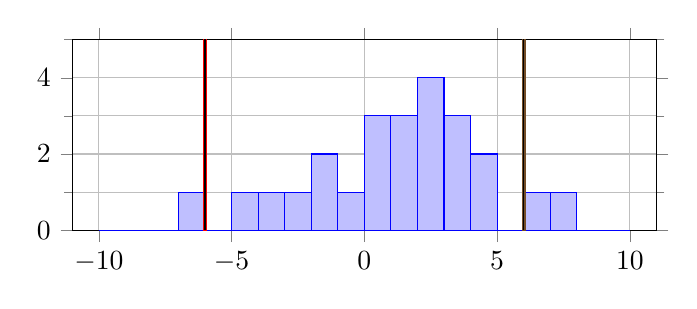
\begin{tikzpicture}
\begin{axis}[
height=4cm,
width=9cm,
%            ybar interval,      % <-- this causes the `xticks' to be centered
ymin= 0, ymax=5,
xmin=-11, xmax=11,
grid=both,
minor y tick num=1,
%yminorgrids=true,
tick align=outside, % <-- this positions the ticks "outside"
]
\addplot+ [
ybar interval,
mark=none,
fill=blue!25,   % fill the bars again
] coordinates {

	(-10,0)	%
	(-9,0)	%
	(-8,0)	%
	(-7,1)	%
	(-6,0)	%1
	(-5,1)	%11
	(-4,1)	%1
	(-3,1)	%111111
	(-2,2)	%1111
	(-1,1)	%11111
	 (0,3)	%111
	 (1,3)	%1
	 (2,4)	%
	 (3,3)	%
	 (4,2)	%
	 (5,0)	%
	 (6,1)	%
	 (7,1)	%
	 (8,0)	%
	 (9,0)	%
	 (10,1)	%

};

\addplot+ [
ybar interval,
mark=none,
fill=black,   % fill the bars again
] coordinates {
	(-6.05,16) 
	(-5.95,16) 
};

\addplot+ [
ybar interval,
mark=none,
fill=black,   % fill the bars again
] coordinates {
	(6.05,16) 
	(5.95,16) 
};
\end{axis}

\end{tikzpicture}
	\caption{Histogram of one sensor face reading the same tag multiple times}
	\label{fig:histogram}
\end{figure}

We did some stuff, wrote it down here...

\begin{figure}[h]
	\begin{tikzpicture}
\begin{axis}[view={-20}{20}, grid=both]
\addplot3[surf] file {data.txt};
\end{axis}
\end{tikzpicture}
       
	\caption{Histogram of one sensor face reading the same tag multiple times}
	\label{fig:histogram}
\end{figure}


%%%%%%%%%%%%%%%%%%%%
\subsection{3D M-Blocks System Experiments}
\label{sec:mblocksExperiments}
We 

\begin{table}[h]
	\caption{Experimental results for }
	
	\begin{tabular}{ p{3.4cm}  p{1.9cm}  p{1.9cm} }
		\hline
								& Attempts 	& Successes \\
		\hline
		Configuration Discovery	&  -1 		& -50 \\
		Direction Following		& 0 		& 0  \\
		command Tags 			&  -1 		& -50 \\


		
	\end{tabular}
	
	\label{tab:info}
\end{table}

